\documentclass{article}

% Set page size and margins
\usepackage[letterpaper,top=1in,bottom=1in,left=1in,right=1in,marginparwidth=1.75cm]{geometry}

% Useful packages
\usepackage{amsmath}
\usepackage{graphicx}
\usepackage[colorlinks=true, allcolors=blue]{hyperref}
\usepackage{subcaption}
\usepackage{natbib}

\title{Accelerate GWAS through Parallel}
\author{Weixiao Zhan}

\begin{document}
\maketitle

\section{Introduction}

The motivation of the project is to address the inefficiencies,
specifically time-latency,
observed in \texttt{plink} computing Genome-Wide Association Studies (GWAS, \cite{uffelmann2021genome}).
Recognizing the computation of GWAS is highly 
parallelizable: effect size ($\beta$) and significance ($p$-value) 
of each Single Nucleotide Polymorphism (SNP) does not depend on 
another's allele frequency,
this project, \textbf{parallel GWAS}, aim to reimplement GWAS 
leveraging hardware parallel capabilities.
In addition, run time comparison between \texttt{plink} and parallel GWAS,
is conducted on two different platforms to evaluate performance.

\section{Methods}
Matrix arithmetic are well implemented in parallel by open-source libraries.
The methodology is to convert GWAS regression problem into matrix arithmetic,
and leverage existing libraries to accelerate computation.
Specifically, parallel GWAS uses PyTorch library by \cite{paszke2019pytorch}.

\subsection{preprocessing}
Firstly, construct allele frequency matrix $X$ and phenotype matrix $Y$ from file using stream IO.
$$
\begin{matrix}X=&\left[ \begin{matrix}&\vdots &\\ \cdots &x_{i,j}\in \left\{ 0,1,2\right\}  &\cdots \\ &\vdots &\end{matrix} \right]  &\begin{gathered}\uparrow \\ i\in \text{sample} \\ \downarrow \end{gathered} \\ &&\\ &\leftarrow j\in \text{SNP} \rightarrow &\\ Y=&\left[ \begin{gathered}\vdots \\ y_{i}\\ \vdots \end{gathered} \right]  &\begin{gathered}\uparrow \\ i\in \text{sample} \\ \downarrow \end{gathered} \end{matrix}
$$
Then, center $X, Y$ at their means:
$$
\begin{aligned}
X_{:,j}&\leftarrow X_{:,j}-\text{mean} \left( X_{:,j}\right) & \forall j \\ 
Y&\leftarrow Y-\text{mean} \left( Y\right)  
\end{aligned} 
$$

\subsection{effect size}
The effect size can be computed as:
$$
\hat{\beta} =\frac{X^{T}Y}{X^{T}X} 
$$

\subsection{significance (p value)}
The null hypothesis $H_0$ is no association between the phenotype and the genotype,
i.e. $\beta = 0$.
Thus the test statistics can be computed as
$$
\begin{aligned}
\text{stat} &=\frac{\hat{\beta } -0}{SE\left( \hat{\beta } \right)  } \\ 
SE\left( \hat{\beta } \right)  &=\text{var}_{(-2)} (Y-\hat{\beta} X)
\end{aligned}
$$
in which, $\text{var}_{(-2)}(\cdot)$ computes the variance with (n-2) correction.

This statistics follows t-distribution with (number of samples -2) degree of freedom.
Thus $p$-value can be computed as:
$$
\begin{aligned}\text{stat} &\sim T_{df=\text{samples} -2}\\ p\text{-values} &=2\int^{-|\text{stat} |}_{-\infty } T_{df=\text{samples} -2}(t)dt\end{aligned}
$$
It is worth mentioning that there is no close formula for t distribution.
The last step to compute $p$-value is performed in batch operations 
using \texttt{scipy} library instead of parallel. 
Later of this report will discuss the effect of different batch sizes.

\section{Results}
The correctness of parallel GWAS result is verified by \texttt{plink} results.

Run time comparison is conducted on a local PC equipped with Nvidia GPU and datahub.
Figure \ref*{fig:local_cpu} and \ref*{fig:local_gpu} shows the runtime 
on local PC using different hardware.
Figure \ref*{fig:datahub} shows the runtime on datahub. 
Since there is no GPU resource available, only CPU version of parallel GWAS is used.

\begin{figure}[h]
      \centering
      \begin{subfigure}[b]{0.32\textwidth}
            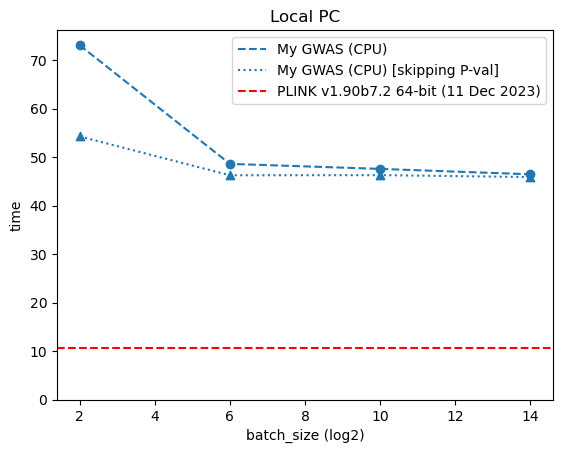
\includegraphics[width=\textwidth]{../local_CPU.png}
            \caption{CPU runtime}
            \label{fig:local_cpu}
      \end{subfigure}
      \begin{subfigure}[b]{0.32\textwidth}
            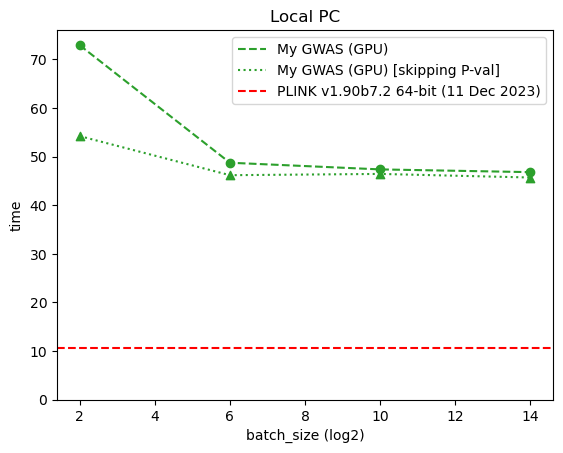
\includegraphics[width=\textwidth]{../local_GPU.png}
            \caption{GPU runtime}
            \label{fig:local_gpu}
      \end{subfigure}
      \begin{subfigure}[b]{0.32\textwidth}
            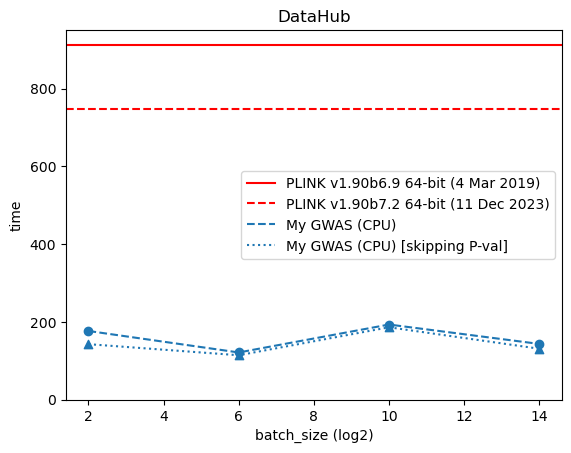
\includegraphics[width=\textwidth]{../datahub.png}
            \caption{\label{fig:datahub}runtime on datahub.}
      \end{subfigure}
      
      \caption{\label{fig:runtime}Runtime comparison}
  \end{figure}


\section{Discussion}
\begin{enumerate}
\item In Figure \ref*{fig:runtime},
the difference between dash and dot line is the time to compute CDF of T distribution.
As the batch size increases, the time computing $p$-values decreases.
However, large batch size may overwhelm the system memory, 
for instance, in Figure\ref*{fig:datahub}, $2^6$ batch size produced peak performance.
Thus batch size is an important parameter to tune on hardware.

\item In Figure \ref*{fig:local_cpu} and \ref*{fig:local_gpu},
runtime difference between CPU and GPU is negligible.
Since GWAS has relatively simple matrix computation,
benefit of having extra parallel cores on GPU 
canceled out with the extra communication cost.

\item Comparing Figure \ref*{fig:local_cpu} and \ref*{fig:datahub},
\texttt{plink} performed dramatically different: $80\times$ faster on local PC.
Potential cause is \texttt{plink 1.9} might used some Intel specific libraries
that are not fully supported by AMD.
Meanwhile, \texttt{plink 2.0}, currently still under development, 
promise to have versions specificity compiled and built AMD, 
which should help speed up calculation on datahub machines in the future.

\end{enumerate}

Future work: 
\begin{enumerate}
\item Add support to handle co-variables, such as 
principle components of population, etc.
\end{enumerate}

\section{Code}
\href{https://github.com/weixiao-zhan/CSE284_ParallelGWAS}
{github repo: https://github.com/weixiao-zhan/CSE284\_ParallelGWAS}

\bibliographystyle{unsrtnat}
\bibliography{references}

\end{document}